% SPDX-FileCopyrightText: 2026 Will Cook
% SPDX-License-Identifier: CC-BY-4.0
% Companion paper on agent-native navigation and proof receipts.
\documentclass[11pt]{article}
\usepackage{paper-house-style}
\usepackage{booktabs,array,float,placeins,multicol,fancyvrb}
\usepackage{tikz}
\usetikzlibrary{arrows.meta,positioning,calc,fit,shapes.geometric}
\usepackage[colorlinks=true,linkcolor=linkinternal,urlcolor=linkexternal,citecolor=linkinternal]{hyperref}
\hypersetup{
  bookmarksnumbered=true,bookmarksopen=true,bookmarksopenlevel=1,
  pdftitle={From a Cold Clone to a Proof Receipt},
  pdfauthor={Will Cook},
  pdfsubject={Agent-native navigation and incremental validation for a large Lean development},
  pdflang={en-GB},
  pdfkeywords={Lean 4, formal mathematics, AI agents, navigation, proof receipts, incremental compilation, reproducibility},
}
\newcommand{\repobase}{https://github.com/wcook04/plectis-lean-erdos249-257}
\DefineVerbatimEnvironment{routeblock}{Verbatim}{
  fontsize=\scriptsize,
  frame=single,
  framerule=0.45pt,
  framesep=5pt,
  rulecolor=\color{MidnightBlue!35},
  xleftmargin=0.02\linewidth,
  xrightmargin=0.02\linewidth
}
% BEGIN generated_semantic_coverage_macros
\newcommand{\SemanticAuthoredTheoremLike}{144,996}
\newcommand{\SemanticAuthoredInterpreted}{139,750}
\newcommand{\SemanticDirectEvidence}{3,263}
\newcommand{\SemanticContextual}{136,487}
\newcommand{\SemanticStructuralOnly}{5,246}
\newcommand{\SemanticAuthoredPercent}{96.4}
% END generated_semantic_coverage_macros
\emergencystretch=1.6em

\runninghead{From a cold clone to a proof receipt}
\title{From a Cold Clone to a Proof Receipt}
\subtitle{Agent-native navigation and incremental validation for a large Lean development}
\author{Will Cook}
\date{July 2026}

\begin{document}
\maketitle
\provenancenote{\emph{Authorship and AI use.} Every word of this manuscript was
generated by agents based on large language models operating within Will Cook's
private research system for artificial intelligence. Cook set the objectives
and acceptance criteria, reviewed and authorised the manuscript, and is
responsible for its contents. The agents are production tools, not authors. See
Appendix~\ref{app:repro}.}

\begin{abstract}
A large formal library can be mechanically exact and still be practically
unreadable to the next human or reasoning agent. This paper presents a
repository architecture that separates first-contact comprehension from proof
checking. At the audited revision, a cold clone exposes a bounded six-line
tour, a mathematical map of ten programmes, a reviewed public claim map with
five explicit open propositions, and an elaborated loaded-root reference graph
joined to source coordinates. These are committed navigation products: they
require no Lean build and make omissions and authority boundaries explicit.
The inventory behind them spans 1,019 Lean modules and 153,253 declarations;
503 of those modules and 8,171 of those declarations are explicitly marked
machine-generated certificate shards, counted as formal source and never as
separate mathematical claims.  The marked figures are a classification
floor, not the generated share: large emitted families predate the markers,
so the true machine-generated share is substantially higher.

Navigation does not receive proof authority. A session notary records an
agent's observations, falsifiable conjectures, abandoned routes, exact Lean
probes, and claims. Probe verdicts come from the pinned Lean process and cannot
be authored by the agent; claims must cite an accepted probe, and replay reruns
the stored bytes. Compilation is similarly separated from orientation. Lake
outputs and content traces support focused or changed-cone builds, while an
exact cached receipt prevents an unchanged dependency-index check from
repeating a full environment export. A dogfood session records six reasoning
notes, one accepted probe, and two claims, and its probe replays at the audited
revision.

The contribution is an authority-preserving composition of exhaustive
inventory, selective interpretation, bounded intent routing, receipted
reasoning, and incremental validation. It is not an autonomous theorem prover,
a portability study, or evidence that the agent's reasoning was optimal or
mathematically novel outside the repository history.
\end{abstract}

\section{The cold-clone problem}\label{sec:problem}

The first interaction with a large Lean repository is usually a filesystem.
The reader sees source files, generated files, scripts, papers, and build
configuration, but not the shape of the mathematics. A language model can
search filenames and text, yet those operations do not answer the questions
that matter: Which programmes exist? Which propositions are established,
conditional, finite, or open? Where does a declaration sit in the formal
dependency graph? Which surface is exhaustive, and which is a human selection?
What may be trusted without compiling anything?

This is not only a convenience problem. When an agent cannot see a library's
option surface, it tends to rediscover existing lemmas, confuse a finite result
with its open unbounded neighbour, or build a new local index because the
existing one was not discoverable. Conversely, loading every declaration,
paper, and proof edge into one prompt destroys the distinctions the extra
context was meant to reveal. A useful first-contact surface must therefore be
small, expandable, and honest about what it omits.

The \href{\repobase}{development studied here} indexes eight open
Erd\H{o}s problems. Problems 249 and 257 are the two principal reviewed
programmes; Problems 68, 243, 251, 269, 1041, and 1049 are problem-owned
expansion lanes with their own notes and explicit nonclaims. The corpus
concentrates its depth around a small number of hard frontiers: exact
separation equivalences for Problem 249, a machine-checked rational
countermodel agreeing with the totient's parity at every index, and
quotient-greedy classifications for Problem 257, with obstruction theorems
recorded beside the routes they close. The generated certificate shards named
in the abstract sit underneath these results as checked finite evidence, not
beside them as further claims. The design goal is not
to replace reasoning with a fixed pipeline. It is to let a capable reader see
enough structure to reason well, while reserving mathematical authority for
the pinned proof kernel.

\section{A layered mathematical option surface}\label{sec:layers}

No single graph can serve all readers without hiding an important distinction.
The repository therefore commits four related layers (Figure~\ref{fig:layers}).
They are projections with different coverage contracts, not successive claims
of understanding.

\begin{figure}[!t]
\centering
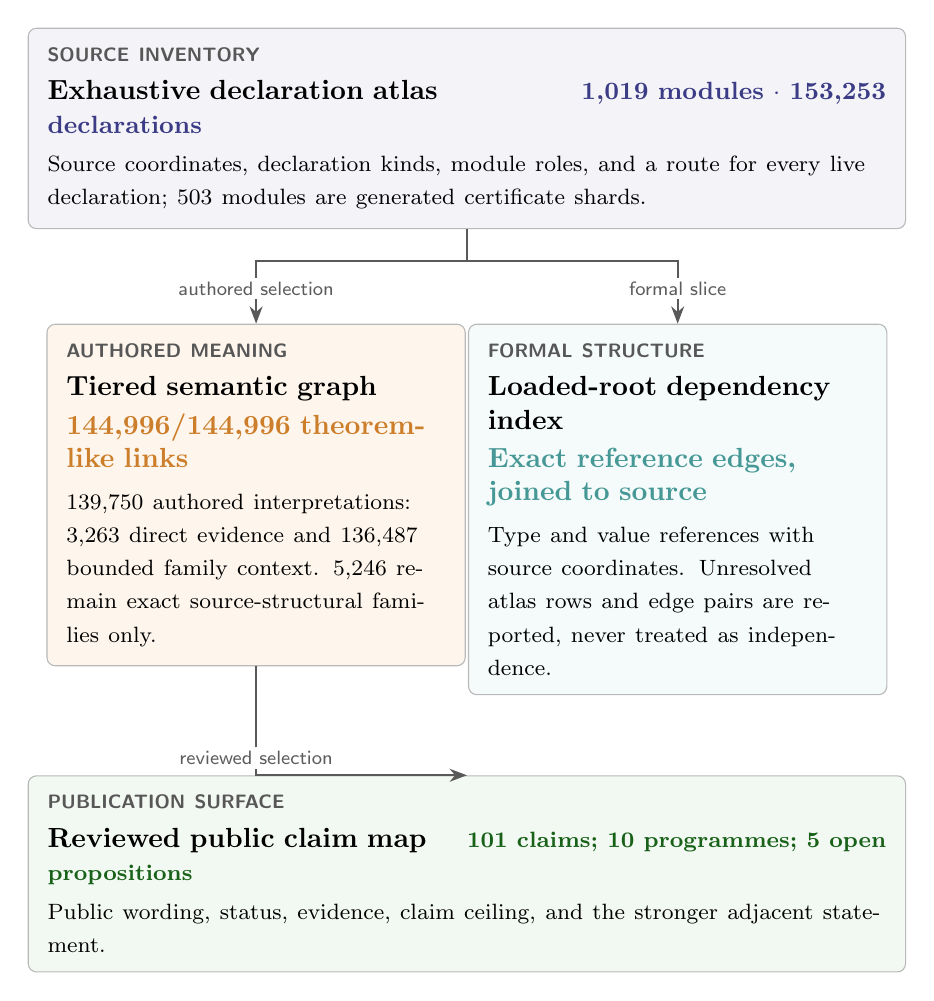
\begin{tikzpicture}[
  wide/.style={draw=gray!55, rounded corners=3pt, align=left, inner sep=7pt,
    text width=10.65cm, fill=white},
  branch/.style={wide, text width=4.82cm, minimum height=3.35cm},
  arr/.style={-{Stealth[length=2.2mm]}, semithick, draw=gray!70!black},
  note/.style={font=\scriptsize\sffamily, text=gray!72!black, fill=white,
    inner sep=1.5pt},
  kicker/.style={font=\scriptsize\sffamily\bfseries, text=gray!68!black}
]
\node[wide, fill=MidnightBlue!5] (atlas) at (0,0)
  {{\scriptsize\sffamily\bfseries\color{gray!68!black} SOURCE INVENTORY}\\[2pt]
   \textbf{Exhaustive declaration atlas}\hfill
   \textcolor{MidnightBlue!85}{\small\textbf{1,019 modules \(\cdot\) 153,253 declarations}}\\[2pt]
   \footnotesize Source coordinates, declaration kinds, module roles, and a route
   for every live declaration; 503 modules are generated certificate shards.};
\node[branch, fill=TealBlue!5, below left=12mm and -5.34cm of atlas.south] (dep)
  {{\scriptsize\sffamily\bfseries\color{gray!68!black} FORMAL STRUCTURE}\\[2pt]
   \textbf{Loaded-root dependency index}\\[2pt]
   \textcolor{TealBlue!75!black}{\textbf{Exact reference edges, joined to source}}\\[3pt]
   \footnotesize Type and value references with source coordinates. Unresolved
   atlas rows and edge pairs are reported, never treated as independence.};
\node[branch, fill=BurntOrange!6, below right=12mm and -5.34cm of atlas.south] (semantic)
  {{\scriptsize\sffamily\bfseries\color{gray!68!black} AUTHORED MEANING}\\[2pt]
   \textbf{Tiered semantic graph}\\[2pt]
   \textcolor{BurntOrange!80!black}{\textbf{\SemanticAuthoredTheoremLike/\SemanticAuthoredTheoremLike\ theorem-like links}}\\[3pt]
   \footnotesize \SemanticAuthoredInterpreted\ authored interpretations:
   \SemanticDirectEvidence\ direct evidence and \SemanticContextual\ bounded
   family context. \SemanticStructuralOnly\ remain exact source-structural
   families only.};
\node[wide, fill=ForestGreen!6, below=12mm of $(dep.south)!0.5!(semantic.south)$] (claims)
  {{\scriptsize\sffamily\bfseries\color{gray!68!black} PUBLICATION SURFACE}\\[2pt]
   \textbf{Reviewed public claim map}\hfill
   \textcolor{ForestGreen!70!black}{\footnotesize\textbf{101 claims; 10 programmes; 5 open propositions}}\\[2pt]
   \footnotesize Public wording, status, evidence, claim ceiling, and the
   stronger adjacent statement.};
\coordinate (fork) at ($(atlas.south)+(0,-4mm)$);
\draw[arr] (atlas.south) -- (fork) -| node[note,pos=.72] {formal slice} (dep.north);
\draw[arr] (fork) -| node[note,pos=.72] {authored selection} (semantic.north);
\draw[arr] (semantic.south) |- node[note,pos=.42] {reviewed selection} (claims.north);
\end{tikzpicture}
\caption{The navigation layers. The dependency index and semantic graph are
different partial views of the exhaustive atlas; neither is presented as a
complete interpretation.}
\label{fig:layers}
\end{figure}

\paragraph{Exhaustive inventory.}
The declaration atlas is a source-derived address book. It records every live
declaration that its explicit source roots contain. Exhaustiveness here means
that a reader can locate a declaration, not that the system understands its
mathematical role.

\paragraph{Exact formal neighbourhoods.}
The dependency index loads the two supported compact roots, extracts direct
constant references from elaborated types and values, and joins those
constants to atlas coordinates. It reports unresolved rows and edges instead
of silently treating absence as independence. Its graph is exact for the
loaded environment and stated edge relation, but it is not a transitive proof
explanation.

\paragraph{Tiered mathematical interpretation.}
The semantic graph contains authored statement nodes, typed relations, and an
exact source-structural floor. At the audited revision all
\SemanticAuthoredTheoremLike\ authored theorem-like declarations are linked.
Of these, \SemanticAuthoredInterpreted\ (\SemanticAuthoredPercent\%) participate
in authored mathematical interpretations: \SemanticDirectEvidence\ are exact
proposition evidence and \SemanticContextual\ are bounded contextual links to
digest- or module-verified families. The remaining \SemanticStructuralOnly\ are grouped only by exact source
module and normalised Lean proposition signature. That lower tier is useful
navigation, not a mathematical paraphrase. Keeping the tiers visible prevents
exhaustive linkage or bulk helper assignment from being misreported as
exhaustive direct understanding. A paper-seeded population query continues to
rank exact live citations whose best route is structural rather than authored.

\paragraph{Reviewed public claims.}
The claim map selects 101 results for public exposition. It records 37 as
proved here, 8 as formalised here, 5 as unconditional progress, 39 as
conditional reductions, 7 as verified finite instances, 3 as cited only, and
2 as open. Five explicit frontier propositions describe the stronger
obligations that survive. These labels are maintainer-reviewed public meaning,
not outputs inferred by the proof kernel.

\section{A bounded tour over an unbounded drilldown}\label{sec:tour}

The first command returns a six-line card rather than a database dump. It
derives corpus scale, formal-graph scale and misses, the authority boundary,
the eight-problem map, the open frontier, and the available intent classes from the committed
projections. The full packet uses a registry-scaled budget: 18\,kB of base
context plus 2\,kB per indexed problem, hence 34\,kB for the present eight-problem
registry. It expands the card into a mathematical map, status counts,
reader-specific contracts, and typed follow-up commands.

Five intent lenses cover the main transitions:
\begin{enumerate}
\item understand the mathematics through a selected programme and its claims;
\item locate any formal object through ordinary-language search followed by
      exhaustive inventory;
\item inspect exact formal dependencies through proof cones and paths;
\item begin a checked change through the session notary and focused builder;
\item audit the agent and release system through the publication architecture
      and release gate.
\end{enumerate}
The route logic names no specimen theorem or module. Repository-specific
mathematics enters through data: programme rows, claims, declaration records,
and frontier propositions. This distinction matters. The mechanism is generic
over the repository's projection schemas, while the current projection content
is intentionally specific to the mathematics it describes.

Ordinary-language entry is likewise not an undocumented trigger list. The
\texttt{--vocabulary} packet is an executable Rosetta surface: it publishes
question operators, aliases, transparent expansions, typed route hints, an
all-problem registry projected from \texttt{docs/problems.json}, and a
route-discovery lexicon projected from
\texttt{docs/claims.json::machine\_readable\_paper.entrypoints}. A unique exact
authored term may take a constant-time fast path; ambiguous or unseen language
falls through to visible vocabulary interpretation and ranked corpus search.
Every search response records that interpretation, so an agent can inspect how
its wording was translated instead of depending on phrase luck.

The packet also answers four different cold readers. A research mathematician
gets programmes, claim statuses, and surviving open propositions. A
formalisation engineer gets declaration coordinates, exact value references,
and a route into a checked change. An AI-lab researcher gets coverage and
authority distinctions. An independent contributor gets the no-build
orientation, changed-cone build route, and public handoff check. Each reader
sees the same facts through a different question contract rather than a
separate hard-coded example.

\section{Crossing from navigation to authority}\label{sec:authority}

The architecture treats navigation and proof as separate capabilities
(Figure~\ref{fig:sequence}). A static query may nominate a theorem or dependency
path. It cannot establish that a proposed application typechecks, that a proof
closes a goal, or that an English interpretation is mathematically faithful.

\begin{figure}[!t]
\centering
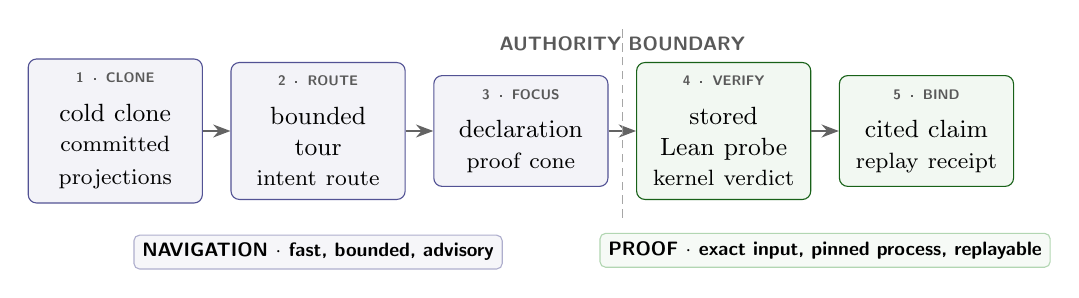
\begin{tikzpicture}[
  stagebox/.style={draw, rounded corners=3pt, align=center, text width=1.86cm,
    minimum height=1.36cm, fill=white, inner sep=5pt},
  exact/.style={stagebox, draw=ForestGreen!70!black, fill=ForestGreen!6},
  nav/.style={stagebox, draw=MidnightBlue!75, fill=MidnightBlue!5},
  arr/.style={-{Stealth[length=2.2mm]}, semithick, draw=gray!78!black},
  step/.style={font=\tiny\sffamily\bfseries, text=gray!70!black},
  phase/.style={draw, rounded corners=2pt, inner sep=3pt,
    font=\scriptsize\sffamily\bfseries}
]
\node[nav] (clone)
  {{\tiny\sffamily\bfseries\color{gray!70!black} 1 · CLONE}\\[3pt]
   \small cold clone\\[-1pt]\footnotesize committed projections};
\node[nav, right=3.5mm of clone] (tour)
  {{\tiny\sffamily\bfseries\color{gray!70!black} 2 · ROUTE}\\[3pt]
   \small bounded tour\\[-1pt]\footnotesize intent route};
\node[nav, right=3.5mm of tour] (cone)
  {{\tiny\sffamily\bfseries\color{gray!70!black} 3 · FOCUS}\\[3pt]
   \small declaration\\[-1pt]\footnotesize proof cone};
\node[exact, right=3.5mm of cone] (probe)
  {{\tiny\sffamily\bfseries\color{gray!70!black} 4 · VERIFY}\\[3pt]
   \small stored Lean probe\\[-1pt]\footnotesize kernel verdict};
\node[exact, right=3.5mm of probe] (claim)
  {{\tiny\sffamily\bfseries\color{gray!70!black} 5 · BIND}\\[3pt]
   \small cited claim\\[-1pt]\footnotesize replay receipt};
\draw[arr] (clone) -- (tour);
\draw[arr] (tour) -- (cone);
\draw[arr] (cone) -- (probe);
\draw[arr] (probe) -- (claim);
\draw[densely dashed, gray!70] ($(cone.east)!0.5!(probe.west)+(0,-11mm)$) --
  ($(cone.east)!0.5!(probe.west)+(0,13mm)$);
\node[font=\scriptsize\sffamily\bfseries, text=gray!70!black,
  above=9mm of $(cone.east)!0.5!(probe.west)$] {AUTHORITY BOUNDARY};
\node[phase, draw=MidnightBlue!35, fill=MidnightBlue!4,
  below=5mm of $(clone.south)!0.5!(cone.south)$]
  {NAVIGATION \(\cdot\) fast, bounded, advisory};
\node[phase, draw=ForestGreen!35, fill=ForestGreen!4,
  below=5mm of $(probe.south)!0.5!(claim.south)$]
  {PROOF \(\cdot\) exact input, pinned process, replayable};
\end{tikzpicture}
\caption{The shortest path from first contact to an authoritative receipt.
The agent chooses the route; the pinned Lean process supplies the verdict.}
\label{fig:sequence}
\end{figure}

The session notary records a typed move grammar in an append-only ledger:
observations, conjectures, plans, interpretations, abandonments, probes,
claims, and closure. Conjectures may declare a falsifier. Dead ends remain in
the record instead of being rewritten into a linear success story.

A probe is different. The notary stores the exact Lean input bytes, runs the
pinned Lean process, and computes one of three verdicts from the process
result: accepted, accepted with an admitted placeholder, or rejected. The
agent cannot type a verdict into the ledger. A claim must cite an accepted
probe receipt; the notary rejects weaker citations. Replay reruns every stored
probe and compares the current result with the recorded verdict.

This design deliberately leaves search policy open. LeanDojo couples an open
programmatic Lean environment with extracted proof data, premise annotations,
retrieval, and a theorem-proving benchmark~\cite{leandojo}. Pantograph exposes
tactic execution, proof states, metavariables, and data extraction through
machine interfaces~\cite{pantograph}. Those systems make machine-to-Lean
interaction richer. The notary here addresses a complementary question: after
an agent chooses its own policy, which parts of the resulting reasoning record
are advisory, and which exact claims are grounded by replayable kernel
acceptance?

\section{Compilation after comprehension}\label{sec:incremental}

A committed navigation projection is portable text; an \texttt{.olean} file is
a toolchain- and platform-specific build product. A cold clone can therefore
orient immediately but must either compile the selected formal target or
restore a compatible cache before editing.

The focused build wrapper accepts an exact target, modules changed since a Git
reference, or the stale cone derived from Lake traces. It orders the selected
modules into dependency waves, limits parallel jobs, and finishes with a
serialized Lake authority check. Restored caches use Lake's content traces
rather than checkout timestamps. In one historical four-file addition, the
planner selected 26 modules in four waves rather than both complete roots; in a
warm two-root dogfood plan it selected no stale modules. The test suite covers
trace freshness, changed-file selection, dependency ordering, bounded
parallelism, failure propagation, and the final authority check.

The exhaustive dependency-index validator is expensive for a different
reason: it traverses the elaborated environment and exports direct
references. After a full export matches the committed index, the validator
writes an exact receipt below the ignored Lake cache. Its key includes every
supported Lean source file, the toolchain and Lake locks, the exporter and
builder inputs, the declaration atlas and generated manifest, the formal-source
release slice of the claim registry, the dependency-extraction helper
definitions, and the committed index bytes. An ordinary check reuses the receipt
only while all inputs and output
remain byte-identical; an explicit full-check mode bypasses it. A changed
formal or exporter input therefore forces a fresh incremental build and full
export, while documentation-only revisions and exact cache restores do not.

This is intentionally conservative. The receipt does not claim that the
environment export itself has become incremental. It prevents unnecessary
repetition when its entire input surface is unchanged. When Lean source
changes, Lake still recompiles only stale dependencies, but the graph exporter
currently scans the supported environment again.

\section{Dogfood receipt}\label{sec:dogfood}

The committed prospective session is a naturalistic use of the workbench, not
a synthetic benchmark. The ledger contains six reasoning notes, one
kernel-accepted probe, and two claims bound to that probe. It produced a binary
carry-pivot normal form for numeral-adjacent boundary words and an exact
divisor-incidence identity that sharpens a previously landed one-sided
coefficient bound to equality. At the audited revision, replay reruns the
stored probe and returns the same accepted verdict.

The receipt supports a narrow statement: the stored input is accepted by the
pinned Lean environment, the cited claims point to that accepted probe, and
the result survives replay at this revision. It does not establish that the
agent's route was optimal, that every candidate was searched, that a bounded
failure is impossible, or that the mathematics is new outside the repository
history.

The navigation surface was dogfooded separately as four audiences. The
research-mathematics route reaches the programme map and explicit frontier;
the formalisation route reaches a source coordinate and exact proof cone; the
AI-lab route exposes exhaustive-versus-selective coverage and receipt
authority; the contributor route reaches a focused build and release check.
Adversarial tests remove or distort each protected transition and require the
cold-clone validator to reject the mutation. This evaluates the declared
first-contact contract, not subjective comprehension.

\section{Relation to prior work}\label{sec:related}

Proof blueprints pair informal plans with named Lean declarations and
author-supplied dependency links.  \texttt{leanblueprint} stores a blueprint
in \TeX{} and its checker only confirms that each named declaration
exists~\cite{leanblueprint}; it neither infers those links nor checks that the
informal and formal statements agree.  LeanArchitect infers formal
dependencies and proof-hole status and exports synchronised blueprint
material~\cite{leanarchitect}. The Carleson project shows a blueprint used as
a large collaboration surface. Its public blueprint split the formalisation
into about 180 claimable tasks, most corresponding to one blueprint lemma;
formalisation feedback produced localized corrections, modifications, and
extensions to the mathematical guide, including a few changes to the general
setup and main theorems~\cite{carleson}. The present tour has a different first-contact role. It
begins after the repository already contains a large corpus, distinguishes
exhaustive inventory from authored interpretation, and routes a reader into
exact dependency and proof-receipt tools.

LeanDojo and Pantograph provide stronger interaction substrates for learned or
scripted theorem proving~\cite{leandojo,pantograph}. This work does not propose
a new proof-search policy. It makes the policy slot explicit and records enough
of an agent-chosen trajectory to separate notes, nominations, rejected probes,
and accepted claims.

Nor is its declaration graph or retrieval route novel in isolation.
LeanGraph extracts typed elaborator-level edges across Lean projects, while a
separate network study analyses Mathlib's multilayer declaration
graph~\cite{theoremgraph,mathlibnetwork}. LeanExplore combines semantic,
lexical, and graph ranking behind Python and MCP interfaces, and LeanSearch v2
targets global premise sets through iterative
sketch--retrieve--reflect~\cite{leanexplore,leansearchv2}. The narrower claim
here is that one cold-clone contract composes source addresses, selective
semantics, dependency cones, incremental validation, and authority receipts
without requiring a hosted service or an initial Lean build.

Large-library maintenance supplies the relevant compilation lesson.
\emph{Growing Mathlib} describes performance-aware library design,
deprecation, semantic linters, benchmarks, review tooling, and explicit
technical-debt management~\cite{growingmathlib}. The changed-cone planner and
receipt cache apply a smaller-scale version of that maintenance posture. The
local measurements do not transfer Mathlib's scale or social evidence.

Lean Atlas narrows the declarations whose meaning can affect selected theorem
statements and leaves semantic verification to people~\cite{leanatlas}. That
is close to the authority distinction here: formal dependency can focus human
inspection without deciding intended meaning. The cold-clone tour adds a
front-door contract across exhaustive inventory, selective semantics, public
claims, and agent receipts.

\section{Limits and transfer conditions}\label{sec:limits}

This is a case study of one repository at one audited revision. Its projection
schemas and routing engine are reusable mechanisms, but another project must
supply its own source roots, programme map, claim vocabulary, frontier
statements, and authority owners. The paper gives no evidence that a new
project can adopt the architecture cheaply or that agents using it outperform
agents with an ordinary README.

Counts describe artifact coverage, not mathematical understanding. Direct
dependency edges are not proof explanations. Authored semantic nodes may be
wrong or incomplete. Maintainer-reviewed claims may also be wrong; automation
preserves recorded relationships but does not judge unrestricted prose.

Receipted reasoning is auditable rather than necessarily good. A model may
choose unproductive probes, omit a relevant source, or rationalise a dead end.
Replay detects environment drift in stored probes but not every flaw in the
surrounding interpretation. Context-blind historical experiments also cannot
establish training-data blindness.

Finally, the first full project build and the first elaborated graph export
remain material costs. The architecture moves them after comprehension,
supports compatible cache restoration, and avoids repeating an exact export
when nothing relevant changed. It does not eliminate the cost of validating a
genuinely changed formal environment.

\section{Authority-preserving agent entry}\label{sec:conclusion}

An agent-native formal repository should not merely contain many proofs. It
should reveal, from a cold clone, what mathematics exists, what each navigation
layer knows, what remains open, and which next action crosses into proof
authority. The architecture here realises that sequence with committed
projections, a bounded intent tour, exact loaded-root dependency data, a
session notary, focused builds, and cache-bound validation receipts.

The central design choice is separation. Comprehension comes before
compilation; nomination comes before application; reasoning notes remain
distinct from kernel verdicts; exhaustive routing remains distinct from
selective interpretation; and a public claim remains distinct from the formal
statement it describes. Those boundaries let a capable agent move quickly
without making speed look like authority.

\appendix
\section{Reproduction routes}\label{app:repro}

\paragraph{Declaration of generative AI use.} Every word of this manuscript was
generated by agents based on large language models operating within Will Cook's
private research system for artificial intelligence. The formal proofs and
repository software were likewise drafted and revised by the agents through
that system under Cook's direction. Cook set the objectives and acceptance
criteria, selected and reviewed the public claims, and approved the published
version. Cook assumes responsibility for the accuracy, interpretation, and
presentation of the work. Generative systems are production tools, not authors,
and supply no independent authority.

The public repository commits the tour, route, projections, workbench session,
and validators used in this paper. The shortest reproduction route has three
bounded tasks.

\paragraph{1. Orient without elaborating Lean.}
These commands inspect committed projections only:
\begin{routeblock}
python3 scripts/query_corpus.py --tour --format card
python3 scripts/query_corpus.py --route agent_native_corpus_navigation
python3 scripts/query_corpus.py --search <ordinary-language-query>
python3 scripts/query_semantic.py inventory <candidate-name> --limit 1
python3 scripts/check_cold_clone_comprehension.py --quick
\end{routeblock}
The full tour packet is obtained by omitting the format flag. A declaration
name returned by inventory can be expanded into a direct neighbourhood or
bounded proof cone.

\paragraph{2. Cross into proof authority.}
Beginning formal work enters the notary and then the focused builder:
\begin{routeblock}
python3 scripts/proof_workbench.py open --help
python3 scripts/lean_fast_build.py --jobs 2 --lake-staleness <target>
\end{routeblock}

\paragraph{3. Audit dependency-index reuse.}
The ordinary check may reuse an exact cache receipt; the full check bypasses it:
\begin{routeblock}
python3 scripts/test_lean_dependency_index_cache.py
python3 scripts/build_lean_dependency_index.py --check
python3 scripts/build_lean_dependency_index.py --check --full-check
\end{routeblock}
The first ordinary check after a cold clone may perform the full export; a
matching restored Lake cache can carry the exact receipt. The full-check form
always bypasses it.

\clearpage
{\scriptsize
\begin{multicols}{2}
\begin{thebibliography}{10}
\setlength{\itemsep}{0pt}
\setlength{\parsep}{0pt}
\bibitem{leanblueprint} P.~Massot, \emph{leanblueprint}, plasTeX plugin for
Lean formalisation blueprints, 2020,
\href{https://github.com/PatrickMassot/leanblueprint}{software repository},
accessed 28 July 2026.
\bibitem{leanarchitect} T.~Zhu, P.~Monticone, S.~Welleck, and J.~Avigad,
\emph{LeanArchitect: Automating Blueprint Generation for Humans and AI},
in \emph{17th International Conference on Interactive Theorem Proving},
LIPIcs 382, 2026, pp.~25:1--25:16,
\href{https://doi.org/10.4230/LIPIcs.ITP.2026.25}{DOI}.
\bibitem{carleson} L.~Becker et al., \emph{A Blueprint for the Formalization
of Carleson's Theorem on Convergence of Fourier Series}, 2025,
\href{https://doi.org/10.48550/arXiv.2405.06423}{arXiv:2405.06423}.
\bibitem{leandojo} K.~Yang, A.~M.~Swope, A.~Gu, R.~Chalamala, P.~Song,
S.~Yu, S.~Godil, R.~Prenger, and A.~Anandkumar, \emph{LeanDojo: Theorem
Proving with Retrieval-Augmented Language Models}, in \emph{Advances in
Neural Information Processing Systems 36}, 2023,
\href{https://doi.org/10.48550/arXiv.2306.15626}{arXiv:2306.15626}.
\bibitem{pantograph} L.~Aniva, C.~Sun, B.~Miranda, C.~Barrett, and S.~Koyejo,
\emph{Pantograph: A Machine-to-Machine Interaction Interface for Advanced
Theorem Proving, High Level Reasoning, and Data Extraction in Lean 4}, in
\emph{Tools and Algorithms for the Construction and Analysis of Systems},
2025, pp.~116--137,
\href{https://doi.org/10.1007/978-3-031-90643-5_6}{DOI}.
\bibitem{theoremgraph} S.~Kurgan et al., \emph{TheoremGraph: Bridging Formal
and Informal Mathematics}, 2026,
\href{https://doi.org/10.48550/arXiv.2606.25363}{arXiv:2606.25363}.
\bibitem{mathlibnetwork} X.~Li, N.~Peng, S.~Severini, and P.~Shafto,
\emph{The Network Structure of Mathlib}, 2026,
\href{https://doi.org/10.48550/arXiv.2604.24797}{arXiv:2604.24797}.
\bibitem{leanexplore} J.~Asher, \emph{LeanExplore: A Search Engine for Lean 4
Declarations}, 2025,
\href{https://doi.org/10.48550/arXiv.2506.11085}{arXiv:2506.11085}.
\bibitem{leansearchv2} G.~Gao et al., \emph{LeanSearch v2: Global Premise
Retrieval for Lean 4 Theorem Proving}, 2026,
\href{https://doi.org/10.48550/arXiv.2605.13137}{arXiv:2605.13137}.
\bibitem{growingmathlib} A.~Baanen, M.~R.~Ballard, J.~Commelin,
B.~Gin-ge Chen, M.~Rothgang, and D.~Testa, \emph{Growing Mathlib:
Maintenance of a Large Scale Mathematical Library}, in \emph{Intelligent
Computer Mathematics}, 2025,
\href{https://doi.org/10.48550/arXiv.2508.21593}{arXiv:2508.21593}.
\bibitem{leanatlas} B.~Yanahama and A.~Sannai, \emph{Lean Atlas: An
Integrated Proof Environment for Scalable Human--AI Collaborative
Formalization}, 2026,
\href{https://doi.org/10.48550/arXiv.2604.16347}{arXiv:2604.16347}.
\end{thebibliography}
\end{multicols}
}

\end{document}
